\chapter{Adaboost}

\section{Introduction}

Adaboost (Adaptive Boosting) [\cite{ref94}, \cite{ref95}, \cite{ref112}] belongs to a group of methods, or rather meta-algorithms, that do not focus on optimizing one particular algorithm - instead, Adaboost uses an ensemble of algorithms, which individually do not provide excellent results but, together, give very good results. The main idea is similar to the above mentioned Random Forests algorithm: Simple, slightly above average experts can, together, provide an excellent result by voting and thus overcoming the success of any single smart expert. Adaboost is based on weighting training samples as described lower.

\section{Boosting Principle}
In its ensemble, a boosting meta-algorithm usually employs the same type of an algorithm called weak learner. The weak learner is an algorithm for which it is quite sufficient that (considering two classes) its classification error is arbitrarily less than $50 \%$ (however, this is only a minimal request).

To improve classification results, additional classifiers with the same property are added gradually to upgrade the overall outcome. Each such classifier may work well on only 'its own' randomly selected part of the training samples, while leaving other samples to colleagues - the ensemble's classification ability is thus enhanced.

The starting requirement is the determination of the number of weak learners, $n_{w l}$ which is related to the random division (by bagging, for example) of the\\
training set into the appropriate number of training subsets, $n_{w l}$ one for each learner.

There is no unambiguous algorithm to determine the value of $n_{w l}$ in advance. The general requirement is that every sample from the training set $D$ is involved in the training process and further, the number of training samples for each learner would be approximately the same, given that every learner has an equal vote in the final voting. Each trained learner then provides its classification of an unlabeled item and the result is given by majority.

The principle is quite simple, but it has, unfortunately, some difficulties in practice. Easier classifying tasks are typically characterized by the fact that the first trained classifier just works correctly on the vast majority of samples $m_{1}$, where $m_{1} \gg m_{i}, i=2 \ldots, n_{w l}$. The assumption that only a small number of samples remains to be covered by the following necessary classifiers to complete the task results in insufficient training due to the lack of training samples. As a consequence, not all training samples available in $D$ are used and the result is not optimal, given the circumstances.

The applied solution is usually to repeat the whole boosting procedure a few times to ensure the best value for $m_{1}$, approximately equal distribution of number of samples in training subsets, and, if possible, utilization of all training samples. In order to do this, various heuristics are used to try to keep up requirements.

\section{Adaboost Principle}
Nowadays, \textit{Adaptive Boosting} is probably the most widely used boosting option. It allows the addition of weak learners until a certain desired low classification error value is reached. Each training sample is given a weight which determines the probability of its selection from $D$ into the training subset of each individual classifier from the created ensemble. If a training sample is classified correctly, its chances of re-selection by the following classifier decrease; otherwise it grows. Thus, Adaboost focuses on difficult samples.

Initially, the samples receive the same weight value. In every iteration step $k, 1 \leq k \leq k_{\text {max }}$, a particular training set is generated by the sample selection based on the weights which the probability of being selected. Each classifier, $C_{k}$, is trained on its $k$ 's set.

In the next step, with the help of $C_{k}$, the weights of incorrectly classified samples are increased and weights of samples classified correctly are reduced.

In line with their weights and based on the new selection probability distribution, the remaining samples are then used to create another classifier $C_{k+1}$, and the process continues iteratively until the predetermined maximum number of weak learners, $k_{\text {max }}$, is reached, no next training samples are available, or the lowest desired classification error of the ensemble is reached.

\begin{figure}[H]
\begin{center}
  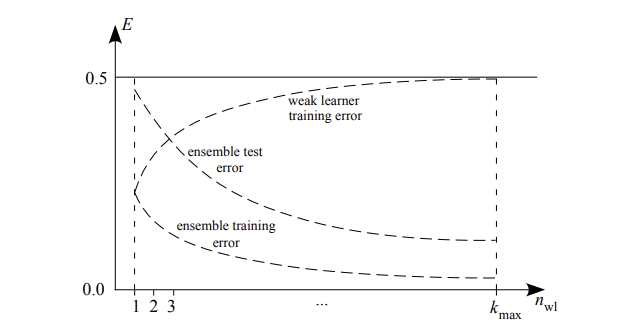
\includegraphics[width=0.8\textwidth]{chapter/chapter9/figure9_1.png}
\caption{The classification error of a classifying ensemble depending on the number of weak learners.}
\label{fig9.1}
\end{center}
\end{figure}

Figure 9.1 illustrates the typical progress of the training process with the gradual addition of more and more weak learners (the axis $n_{w l}$ ). The first weak learner shows the highest classification error $E$ (recall that it must be always less than $50 \%$ for two classes) on both training and test data. After adding another weak learner (that focuses on samples not mastered by previous weak learners), the overall error of the ensemble always drops somewhat on both the training and test data, although the error rate of the gradually added individual weak learners typically progressively increases due to their focus on increasingly difficult examples. As long as every weak learner works with an error value less than $50 \%$, the weighted decision by the entire voting ensemble guarantees a drop in error on the training data, and commonly on the testing data as well.

In theory, the presented curves represent an exponential decrease and increase in error values.

In any case, it is necessary to be cautious because increasing the number of classifiers $k_{\text {max }}$ in an ensemble can lead to undesirable over-training (loss of ability to generalize due to overfocusing of classifiers to recognize only "their" specific training data). However, many simulation experiments have shown that this rarely happens, even for extremely high values of $k_{\text {max }}$.

A brief and well-explained issue of the Adaboost method can be found, for example, in [\cite{ref76}]. To summarize, the following empirical basic rule applies to the practical application of Adaboost:

Boosting improves classification only if individual classifiers in an ensemble provide better than just random results - unfortunately, this cannot be guaranteed in advance.

Despite the absence of a priori guarantee, the method provides very good results in many real-world problems, which is why it is so popular today and used frequently, represented by various implementations, including R.

\section{Weak Learners}
What classification algorithm should be used as a weak learner? Given the basic requirement for a weak learner to achieve better than completely random results, choosing the right algorithm is not critical. Most implementations, including the one demonstrated here in R , use decision trees, especially their simplest variant known as stump.

The stump algorithm, as its name indicates, is a tree limited to the root node from which the branches lead directly to the leaves. The root contains a test for the value of one of the attributes, preferably one that reduces as much as possible the heterogeneity of a set containing a mixture of examples from different classes. Hence, a better than random selection results in more homogeneous subsets.

Note that it is not excluded that some stumps may share the same attribute. In such cases, the root can test the shared attribute using the same or quite different values, depending on the specific situation.

Figure 9.2 shows an example of the stump-tree. For a given task, one of the available attributes, $x_{i}$, is chosen to decide which label should be assigned to a classified item, based on the specific value of that $x_{i}$.

Because the attribute classification relevance may change during the gradual addition of weak learners (as well as the removal of examples from the original training set), different stumps arise in terms of the tested attributes in the roots. Hence, it may also be an advantage that the list of such attributes is a secondary (or eventually might be even primary) result of the classification, thus contributing to the knowledge extracted from the analyzed data.

The unquestionable advantage of using stumps is that due to their simplicity they do not need long and complicated training. Given the principles of the Adaboost method, the desired result can be achieved simply by using a sufficient amount of stumps, which naturally depends on a sufficient number of quality training samples covering the required classes.

Figure 9.3 illustrates the Adaboost-based process of classification. Gradually, $k_{\text {max }}$ stumps were trained using $k_{\text {max }}$ mutually disjunctive subsets of the original set of training samples.

Having two classes, each stump uses one of the attributes for its decision on whether the unlabeled item belongs to class $\mathrm{C}_{1}$ or $\mathrm{C}_{2}$. The final decision is given by voting majority.

\begin{figure}[H]
    \centering
  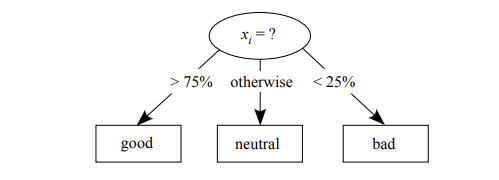
\includegraphics[width=1\textwidth]{chapter/chapter9/figure9_2.png}
\caption{An example of stump. The root tests the attribute $x_{i}$ and, according to the result, assigns one of three possible classes to an unlabeled item.}
\label{fig9.2}
\end{figure}

\begin{figure}[H]
\begin{center}
  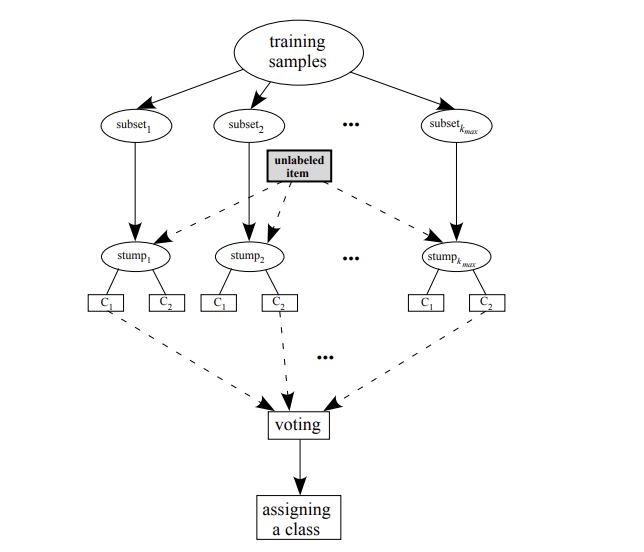
\includegraphics[width=0.8\textwidth]{chapter/chapter9/figure9_3.png}
\caption{The illustration of training and classification by Adaboost.}
\label{fig9.3}
\end{center}
\end{figure}

\section{Adaboost in R}
The demonstrated application of Adaboost uses the library called ada, which must first be installed. The results of two different tree-based weak learners are\\
shown for the purpose of illustration: a decision tree (the rpart library, Recursive Partitioning and Regression Trees), and stump (in the R-code below, see the variable maxdepth $=1$ for stump).

The R code for running the described Adaboost meta-algorithm:
\begin{verbatim}
library(ada)
library(rpart)
# loading the data
data <- read.csv('BookReviews.csv', header=TRUE)
# converting the data to a matrix
dtm <- as.matrix(data)
# removing the object data (unnecessary from now)
rm(data)
# number of instances
n <- dim(dtm)[1]
# number of attributes
m <- dim(dtm)[2]
# indexes of 100 testing samples
number_of_test_samples <- 100
test_index <- sample(n, number_of_test_samples)
# selecting training samples
train_data <- dtm[-test_index, 1:(m-1)]
train_labels <- dtm[-test_index, m]
# selecting testing samples
test_data <- dtm[test_index, 1:(m-1)]
test_labels <- dtm[test_index, m]
result <- NULL
for (it in c(1, 5, seq(10, 100, 10))) {
    # with trees
    ada_model <- ada(as.data.frame(train_data),
        train_labels,
        type="real",
        iter=it,
\end{verbatim}

\begin{verbatim}
    nu=0.05,
    bag.frac=1)
predictions_ada <- predict(ada_model,
            as.data.frame(test_data),
            type="vector")
# with stumps
ada_model_st <- ada(as.data.frame(train_data),
    train_labels,
    type="real",
    iter=it,
    nu=0.05,
    bag.frac=1,
    # rpart.control for stumps
    control = rpart.control(maxdepth=1,
            cp=-1, minsplit=0, xval=0))
predictions_ada_st <- predict(ada_model_st,
            as.data.frame(test_data),
            type="vector")
# creating confusion matrices
cm_ada <- table(test_labels, predictions_ada)
cm_ada_st <- table(test_labels, predictions_ada_st)
# number of instances
n <- sum(cm_ada)
# number of correctly classified instances for each class
correct_ada <- diag(cm_ada)
correct_ada_st <- diag(cm_ada_st)
# numbers of each class predictions
class_predictions_ada <- apply(cm_ada, 2, sum)
class_predictions_ada_st <- apply(cm_ada_st, 2, sum)
# accuracy
accuracy_ada <- sum(correct_ada)/n
accuracy_ada_st <- sum(correct_ada_st)/n
# precision per class
precision_ada <- correct_ada/class_predictions_ada
precision_ada <- round(precision_ada, 4)
precision_ada_st <- correct_ada_st/class_predictions_ada_st
\end{verbatim}

\begin{verbatim}
    precision_ada_st <- round(precision_ada_st, 4)
    # storing the results of current iteration
    result <- rbind(result,
        data.frame(it, accuracy_ada, accuracy_ada_st,
                precision_ada["1"],
                precision_ada["0"],
                precision_ada_st["1"],
                precision_ada_st["0"]))
}
# printing classification performance measures
# for individual iterations
rownames(result) <- NULL
colnames(result) <- c("It.",
            "Acc1", "Acc2",
            "Prec1(pos)", "Prec1(neg)",
            "Prec2(pos)", "Prec2(neg)")
print(result)
# plotting the development of classification errors
plot(ada_model)
plot(ada_model_st)
# printing the model information and final confusion
# matrix for submitted training data
print("Adaboost with trees ")
print(ada_model)
print('Adaboost with stumps ')
print(ada_model_st)
\end{verbatim}

The values of classification performance metrics for the adaboost algorithm with trees and stumps will appear on the output (Acc1, Prec1 etc. are the values for the algorithm with trees, the names ending with 2 are related to the algorithm with stumps):

\begin{center}
\begin{tabular}{lrrrrrrr}
 & It. & Acc1 & Acc2 & Prec1(pos) & Prec1(neg) & Prec2(pos) & Prec2(neg) \\
1 & 1 & 0.63 & 0.49 & 0.6731 & 0.5833 & 0.5370 & 0.4348 \\
2 & 5 & 0.63 & 0.52 & 0.6667 & 0.5870 & 0.5686 & 0.4694 \\
3 & 10 & 0.68 & 0.58 & 0.7170 & 0.6383 & 0.6512 & 0.5263 \\
4 & 20 & 0.67 & 0.61 & 0.7115 & 0.6250 & 0.6600 & 0.5600 \\
5 & 30 & 0.68 & 0.63 & 0.7347 & 0.6275 & 0.6731 & 0.5833 \\
6 & 40 & 0.72 & 0.66 & 0.7755 & 0.6667 & 0.6909 & 0.6222 \\
\end{tabular}
\end{center}

\begin{center}
\begin{tabular}{lrrrrrrr}
7 & 50 & 0.70 & 0.69 & 0.7551 & 0.6471 & 0.7069 & 0.6667 \\
8 & 60 & 0.76 & 0.69 & 0.7925 & 0.7234 & 0.7000 & 0.6750 \\
9 & 70 & 0.74 & 0.67 & 0.7843 & 0.6939 & 0.6833 & 0.6500 \\
10 & 80 & 0.73 & 0.68 & 0.7800 & 0.6800 & 0.6885 & 0.6667 \\
11 & 90 & 0.74 & 0.70 & 0.7843 & 0.6939 & 0.6984 & 0.7027 \\
12 & 100 & 0.75 & 0.69 & 0.7885 & 0.7083 & 0.6935 & 0.6842 \\
\end{tabular}
\end{center}

An interested reader can also look at additional output information which, while not presented here, can be seen on the RStudio console after the end of computation. In addition, two graphs (see RStudio, Plots, in the lower right quarter of console) created by the commands plot(ada\_model) for the tree and plot(ada\_model\_st) for the stump are available. The graphs in Figure 9.4 and Figure 9.5 demonstrate the course of classification errors for the training samples during iterations.

\begin{figure}[H]
\begin{center}
  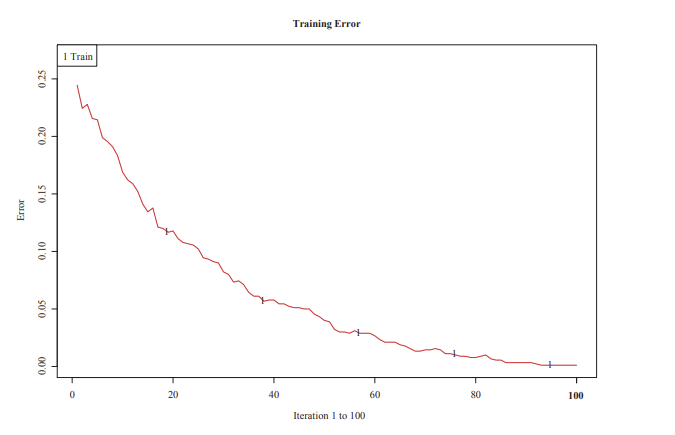
\includegraphics[width=0.8\textwidth]{chapter/chapter9/figure9_4.png}
\caption{Adaboost with trees: the iterative accuracy error reduction.}
\label{fig9.4}
\end{center}
\end{figure}

\begin{figure}[H]
\begin{center}
  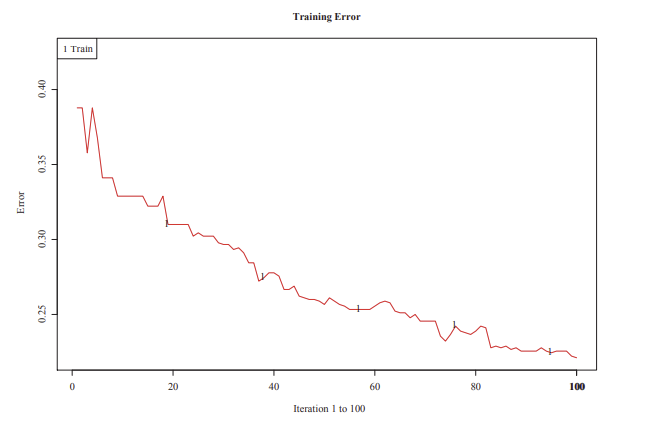
\includegraphics[width=0.8\textwidth]{chapter/chapter9/figure9_5.png}
\caption{Adaboost with stumps: the iterative accuracy error reduction.}
\label{fig9.5}
\end{center}
\end{figure}

It is evident that the full tree works better than the simpler stump; however, in the end, the resulting classification accuracy for the tree variant ( $75 \%$ ) is only $6 \%$ better than that for the stump ( $69 \%$ ). As can be seen here, the stump suffers from poor classification of negative samples, which should perhaps be refined in order to match the positive samples from the information point of view.